\section{Caset: vad är Atlas Copco värt?}
\label{sec:case}

Det här kapitlet går igenom projektets case steg för steg. Alla tal är desamma som i
\kod{docs/case_report.md} och kommer från en körning av \kod{notebooks/case_atco.ipynb} mot
de data som ligger i repot: kurs 192,25\kr{} per den 13 november 2026 och bokslut för 2025.
Kort svar: metoderna ger 116 till 178\kr{} per aktie. Kursen ligger över det, och det
intressanta är varför.

\subsection{Bolaget och datat}

Atlas Copco är en svensk industrikoncern som Yahoo placerar i sektorn Industrials och branschen
Specialty Industrial Machinery. Datat visar ett stort och lönsamt bolag med jämna marginaler.
Omsättningen 2025 var 168~mdkr, EBITDA 44~mdkr och nettovinsten 26~mdkr. Börsvärdet är
938~mdkr och nettoskulden bara 12~mdkr, så rörelsevärdet är 951~mdkr.

\begin{figure}[ht]
\centering
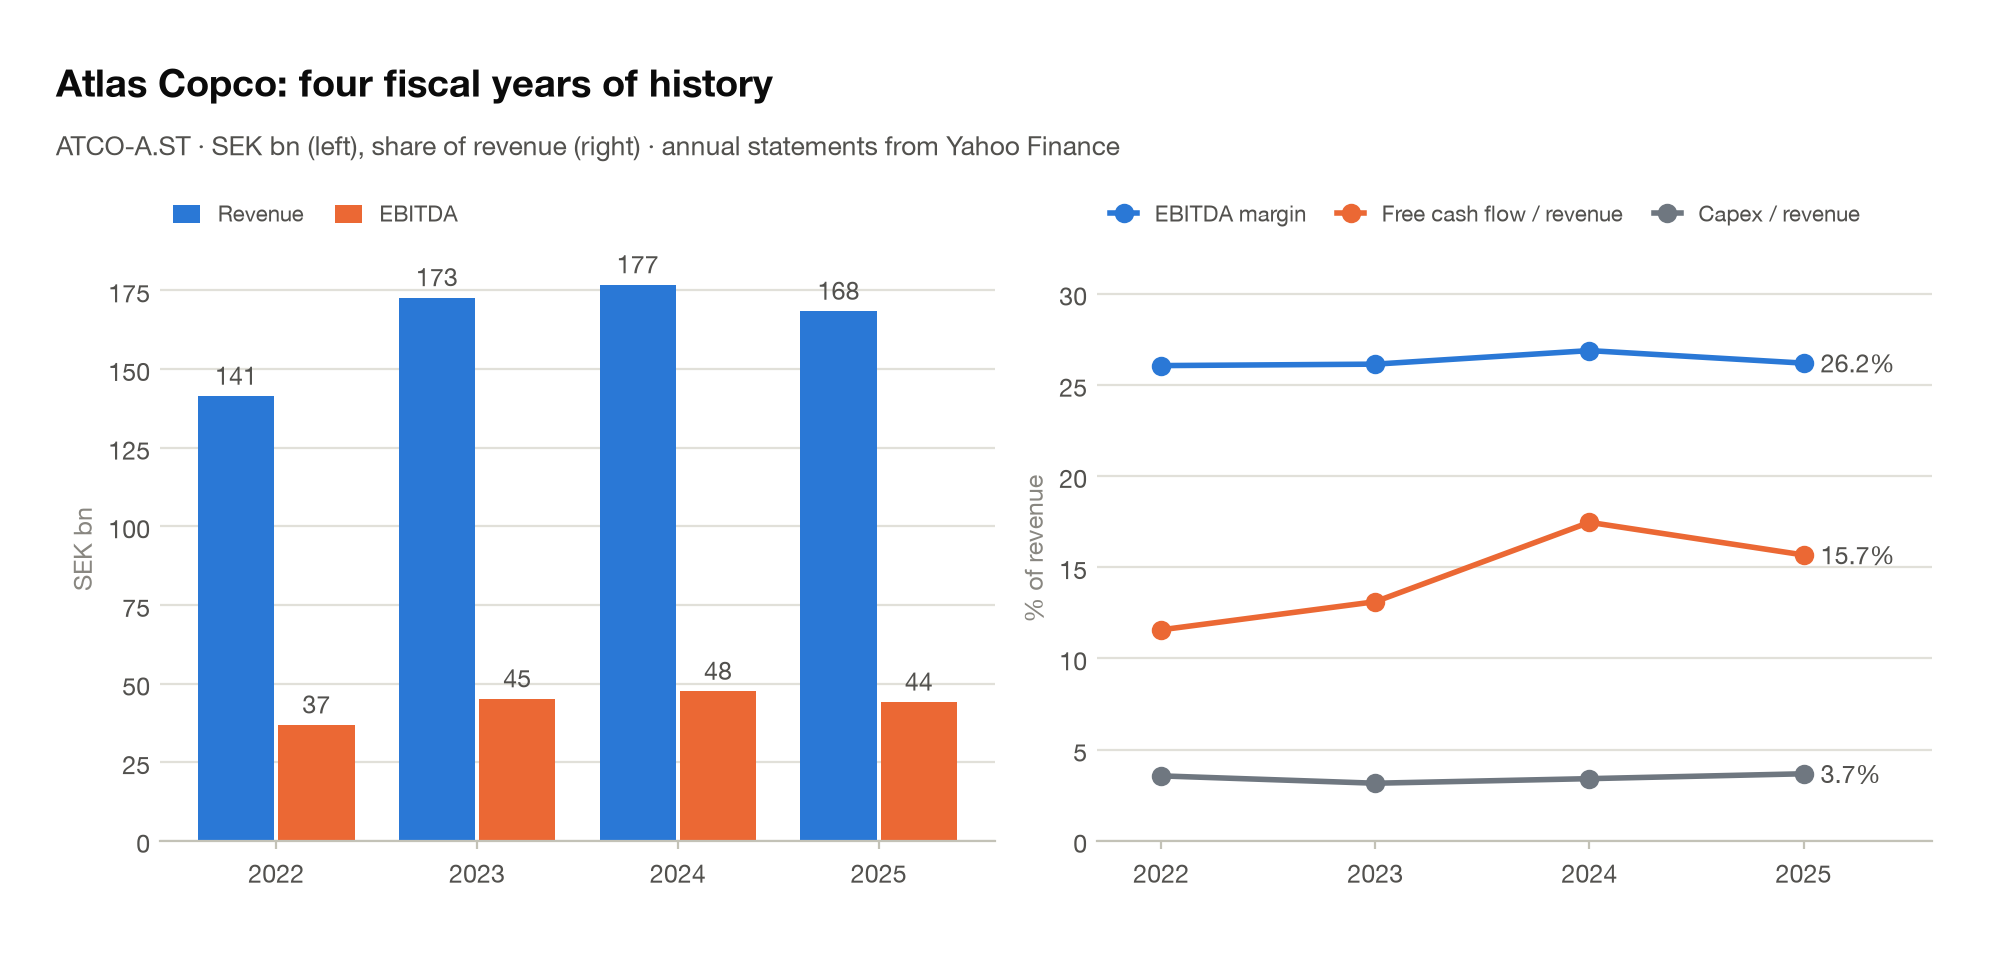
\includegraphics[width=0.95\linewidth]{history_overview.png}
\caption{Atlas Copco 2022 till 2025 enligt projektets datalager.}
\label{fig:historik}
\end{figure}

\begin{table}[ht]
\centering\small
\caption{Historiken som antagandena bygger på.}
\label{tab:historik}
\begin{tabular}{@{}lrrrr@{}}
\toprule
 & 2022 & 2023 & 2024 & 2025 \\
\midrule
Omsättning, mdkr & 141,3 & 172,7 & 176,8 & 168,3 \\
Tillväxt & & 22,2\pct & 2,4\pct & $-4,8$\pct \\
EBITDA-marginal & 26,1\pct & 26,1\pct & 26,9\pct & 26,2\pct \\
Avskrivningar / omsättning & 4,5\pct & 4,5\pct & 5,0\pct & 5,7\pct \\
Capex / omsättning & 3,6\pct & 3,2\pct & 3,4\pct & 3,7\pct \\
Rörelsekapital, smalt mått & 26,9\pct & 25,6\pct & 26,0\pct & 23,9\pct \\
Rörelsekapital, brett mått & 13,8\pct & 13,6\pct & 13,5\pct & 12,8\pct \\
Effektiv skatt & 21,8\pct & 23,0\pct & 21,2\pct & 21,5\pct \\
Förvärv, mdkr & 10,6 & 4,3 & 7,4 & 11,6 \\
\bottomrule
\end{tabular}
\end{table}

Två saker i tabell~\ref{tab:historik} styr resten. Tillväxten är ojämn: nästan hela ökningen
sedan 2022 kom under ett enda år. Och bolaget köper andra bolag för 4 till 12~mdkr om året,
vilket syns i omsättningen men inte i capex.

Tre tidpunkter blandas dessutom i datat. Kursen är från den 13 november 2026, skuld och kassa
från den 30 september 2026 och resultatet från helåret 2025. Yahoos rullande
tolvmånaderssiffror, som motorn inte använder, visar en omsättning på 176~mdkr, 4,7\pct{} över
modellens basår.

\subsection{Antagandena}

Motorns standardantaganden står i tabell~\ref{tab:prognos} och~\ref{tab:wacc}: tillväxt från
6,0\pct{} ned till 2,0\pct, marginal 26,4\pct, WACC 7,65\pct, exit-multipel 19,4. Caset prövar
vart och ett mot historiken och ändrar två:

\begin{itemize}
  \item \textbf{Rörelsekapitalet} sänks från 25,2 till 13,3\pct{} av omsättningen. Motorns smala
    mått~\eqref{eq:nwc} bortser från övriga rörelseskulder som förskott och upplupna kostnader.
    Det breda måttet ligger stabilt kring 13\pct.
  \item \textbf{Skatten} höjs från 20,6 till 21,9\pct, snittet av de tre senaste årens effektiva
    skatt. En koncern med verksamhet i många länder betalar mer än den svenska skattesatsen.
\end{itemize}

Tillväxten behålls, men den är det svagaste antagandet: 6\pct{} om året är snittet av $+22$,
$+2$ och $-5$\pct, och en del av tillväxten är köpt. WACC rörs inte, eftersom ränta och
riskpremie har namngivna källor och beta 1,13 ligger nära Yahoos egen uppgift (1,07).

\subsection{Resultaten}

\begin{table}[H]
\centering\small
\caption{Värde per aktie i kronor. ”Standard” är motorns antaganden rakt av, ”justerat” är med
de två ändringarna. Kurs 192,25\kr.}
\label{tab:resultat}
\begin{tabular}{@{}lrrrrrrr@{}}
\toprule
 & \multicolumn{3}{c}{Standard} & Bas & \multicolumn{3}{c}{Justerat} \\
\cmidrule(lr){2-4}\cmidrule(lr){6-8}
Metod & låg & bas & hög & mot kurs & låg & bas & hög \\
\midrule
DCF, Gordon-tillväxt & 93,7 & 115,8 & 153,7 & $-40$\pct & 93,6 & 115,9 & 154,1 \\
DCF, exit-multipel & 160,6 & 175,2 & 191,0 & $-9$\pct & 160,9 & 175,5 & 191,4 \\
Comps, EV/EBITDA & 152,8 & 172,9 & 190,7 & $-10$\pct & 152,8 & 172,9 & 190,7 \\
Comps, EV/Sales & 111,7 & 138,6 & 168,8 & $-28$\pct & 111,7 & 138,6 & 168,8 \\
Comps, P/E & 162,8 & 178,3 & 196,5 & $-7$\pct & 162,8 & 178,3 & 196,5 \\
LBO, betalningsförmåga & 104,4 & 117,9 & 135,3 & $-39$\pct & 104,6 & 118,2 & 135,7 \\
Monte Carlo, P10, P50, P90 & 84,3 & 116,7 & 164,9 & $-39$\pct & 83,6 & 116,9 & 165,7 \\
\bottomrule
\end{tabular}
\end{table}

Så läser du intervallen i tabell~\ref{tab:resultat} och figur~\ref{fig:football}. För DCF är
lågt värde WACC plus 1 procentenhet och tillväxt minus 0,5 (eller multipel minus 1,0), och
högt värde tvärtom. För comps är det 25:e percentilen, medianen och 75:e percentilen av
jämförelsebolagens multipel. För LBO är det priset som ger 25, 20 respektive 15\pct{}
årlig avkastning. För Monte Carlo är det 10:e, 50:e och 90:e percentilen. Under de senaste 52
veckorna har kursen rört sig mellan 149,6 och 208,3\kr.

\begin{figure}[ht]
\centering
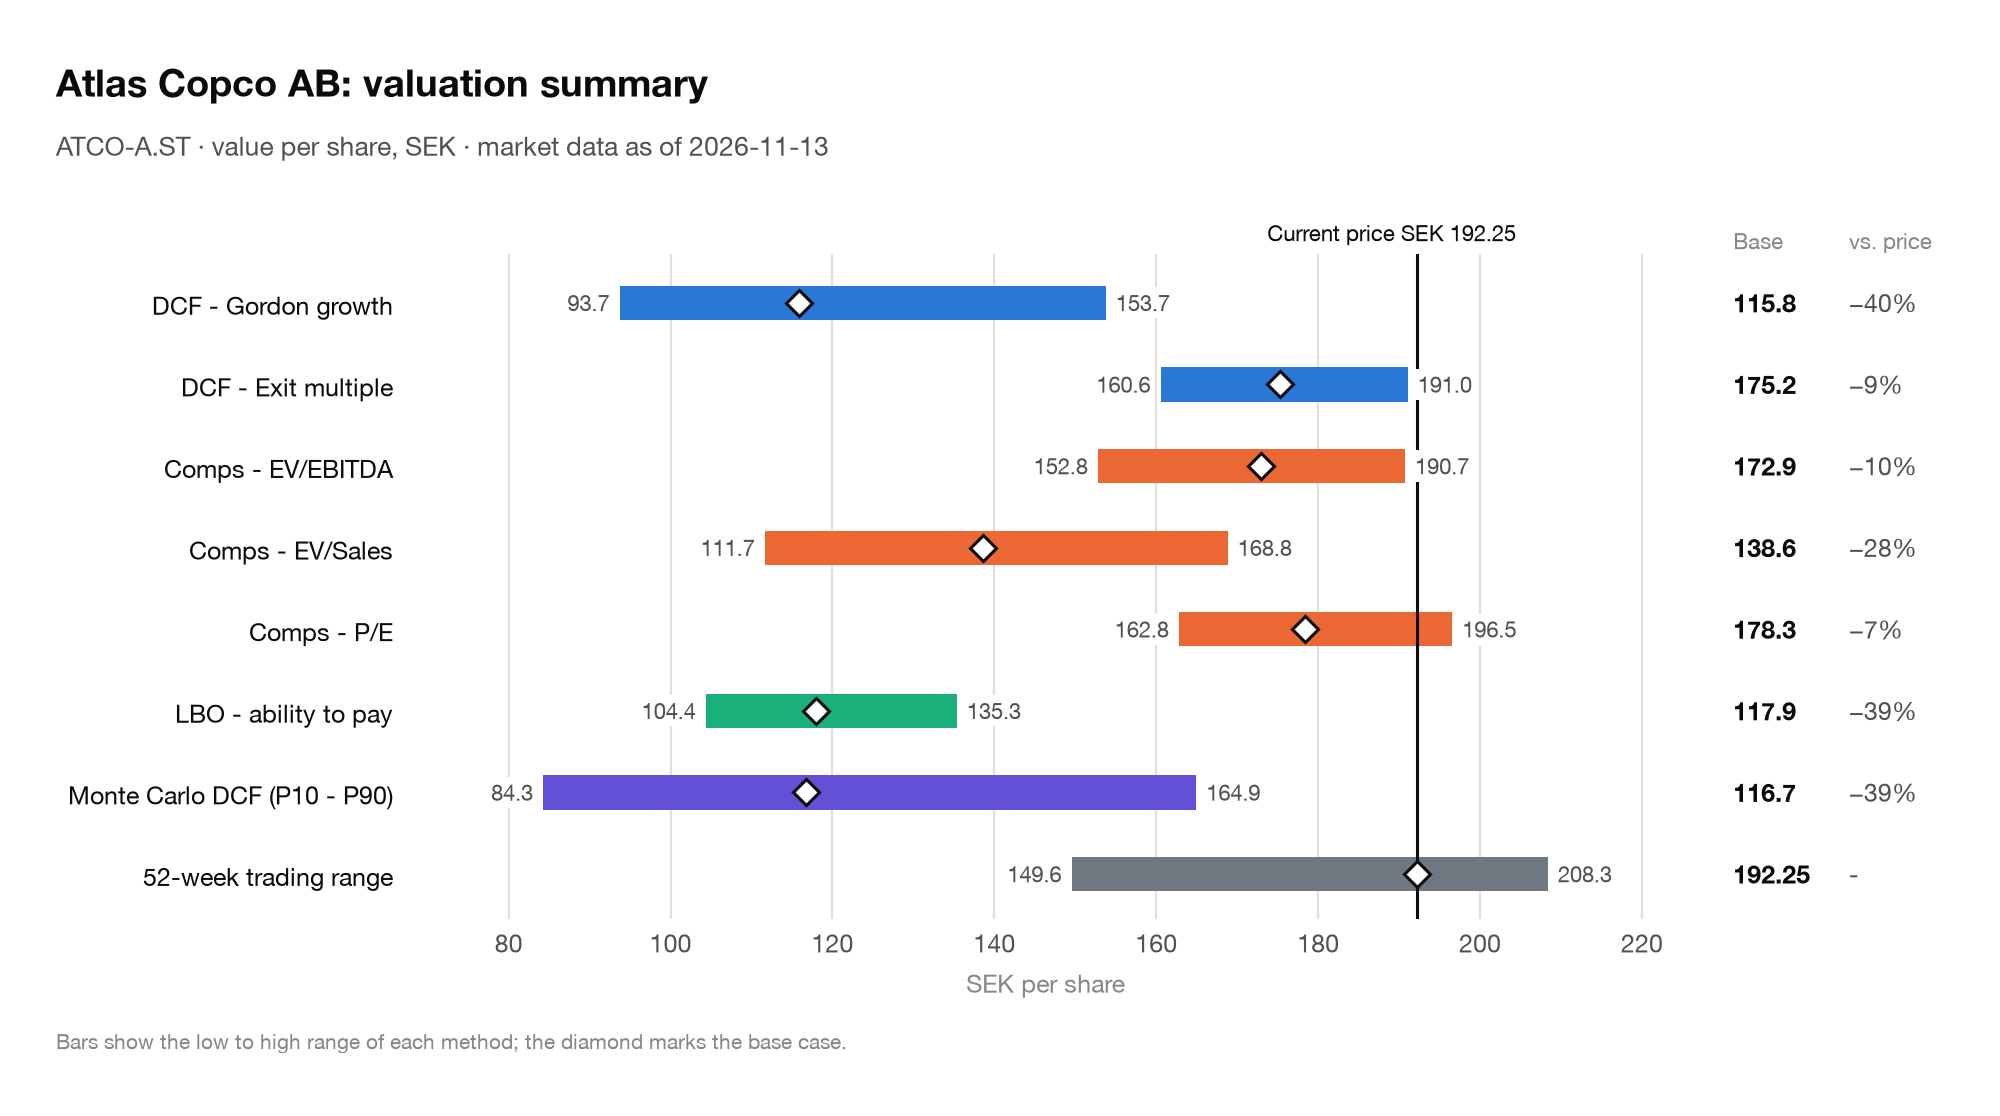
\includegraphics[width=\linewidth]{football_field.png}
\caption{Football field för Atlas Copco med standardantaganden. Staplarna är intervallet per
metod, romben basvärdet och den lodräta linjen kursen.}
\label{fig:football}
\end{figure}

De två justeringarna ändrar nästan ingenting: högre skatt sänker Gordon-värdet med ungefär
2\kr{} och lägre rörelsekapitalbindning höjer det med ungefär 2\kr. Det är i sig ett resultat.
De antaganden som går att pröva mot historiken är inte det som skiljer modellens värde från
kursen.

\subsection{Varför metoderna inte är överens}

Gordon-DCF:en säger 116\kr. Exit-DCF:en och comps säger 173 till 178\kr. Skillnaden sitter i
slutvärdet, som står för 76 till 84\pct{} av hela DCF-värdet:

\begin{itemize}
  \item Gordon-metoden antar 2\pct{} evig tillväxt. Det motsvarar att bolaget om fem år är värt
    11,7 gånger EBITDA.
  \item Exit-metoden antar att bolaget om fem år värderas som jämförelsebolagen i dag, 19,4
    gånger EBITDA. För att Gordons formel ska ge samma slutvärde krävs 4,3\pct{} evig tillväxt.
  \item Comps använder samma bolag och samma multipel direkt: 19,4 gånger EBITDA och 32,9
    gånger vinsten i median. Atlas Copco självt handlas till 21,6 och 35,5.
\end{itemize}

Exit-DCF:en och comps är alltså i grunden samma påstående: bolaget är värt vad marknaden
betalar för liknande bolag. Gordon-DCF:en är det enda oberoende måttet, och det säger att
marknadens multiplar förutsätter mer än modellen antar. Hur mycket mer? Caset räknar baklänges:
vilket värde på en drivare i taget ger exakt dagens kurs?

\begin{table}[H]
\centering\small
\caption{Vad kursen 192,25\kr{} kräver, en drivare i taget.}
\label{tab:baklanges}
\begin{tabular}{@{}lrr@{}}
\toprule
Drivare & Basfall & Krävs för värde = kurs \\
\midrule
WACC & 7,65\pct & 5,39\pct \\
Evig tillväxt & 2,0\pct & 4,6\pct \\
EBITDA-marginal & 26,4\pct & 40,0\pct \\
Snittillväxt år 1 till 5 & 4,0\pct & 16,8\pct \\
Exit-multipel (exit-metoden) & 19,4 & 21,7 \\
\bottomrule
\end{tabular}
\end{table}

Ingen enskild drivare kan rimligen flyttas så långt. Kombinationer räcker längre: WACC
6,24\pct{} tillsammans med 3,0\pct{} evig tillväxt ger precis dagens kurs, liksom 6,67\pct{} med
3,5\pct{} (figur~\ref{fig:implied}). Marknaden prissätter alltså Atlas Copco som om
avkastningskravet vore ungefär 1,4 procentenheter lägre och den eviga tillväxten 1
procentenhet högre än i modellen. Det behöver inte vara fel. En prognos som bromsar till
2\pct{} redan år fem är snål mot ett bolag med stabila marginaler: med tio års inbromsning i
stället för fem stiger Gordon-värdet från 116 till 127\kr. Modellen kan inte avgöra vem som
har rätt, bara visa vad kursen kräver.

\begin{figure}[ht]
\centering
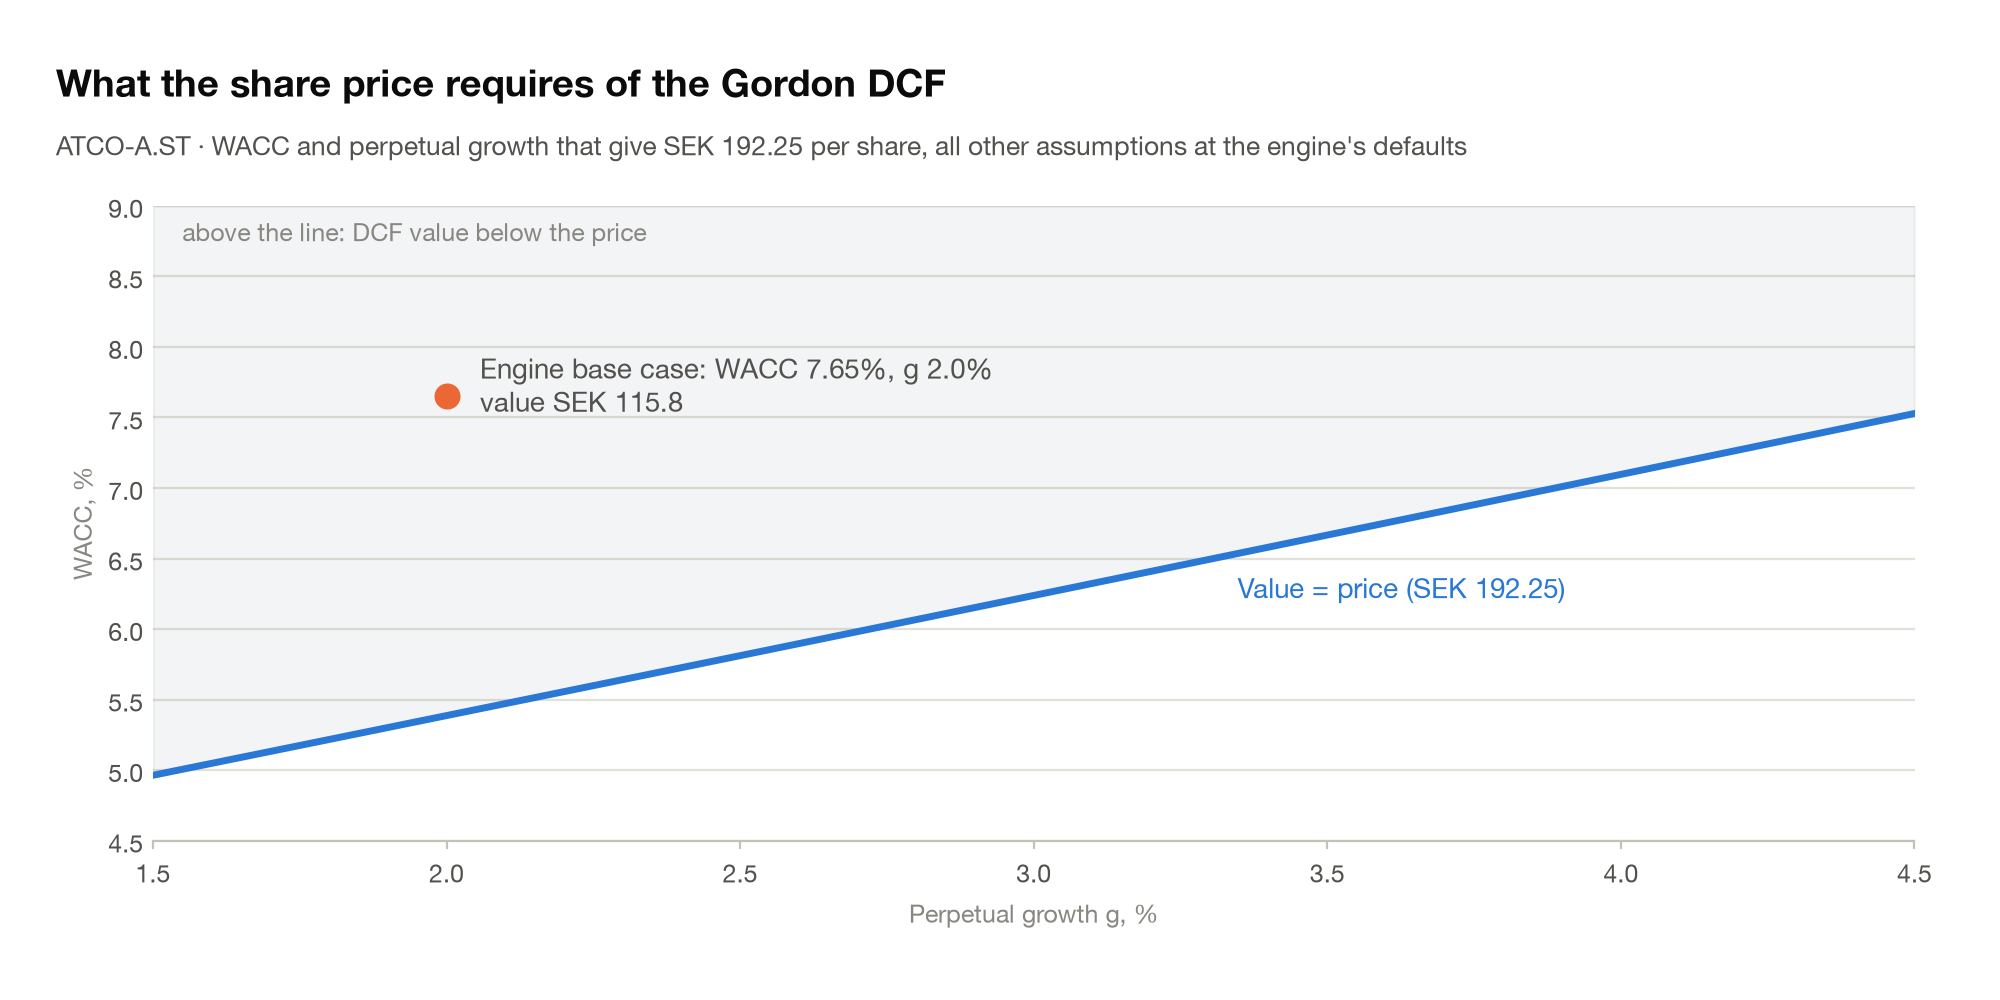
\includegraphics[width=0.9\linewidth]{implied_wacc_growth.png}
\caption{Kombinationer av WACC och evig tillväxt som ger dagens kurs.}
\label{fig:implied}
\end{figure}

De två sista metoderna har egna förklaringar. EV/Sales (139\kr) ligger lågt eftersom en
omsättningsmultipel inte tar hänsyn till att Atlas Copcos marginal (26,2\pct) är högre än
jämförelsebolagens median (21,1\pct). LBO-värdet (118\kr) ligger nära Gordon-DCF:en eftersom
det är samma kassaflöden, se avsnitt~\ref{sec:lbo}.

\subsection{Slutsatsen}

\textbf{Värdeintervall 116 till 178\kr{} per aktie mot kursen 192,25\kr.} Den nedre änden är
Gordon-DCF:ens basvärde i det justerade fallet, den övre basvärdet från P/E-comps. Caset väger
Gordon-DCF:en till 50\pct{} (den enda metoden som inte lånar sin värdering från dagens
börskurser) och comps på EV/EBITDA och P/E till 25\pct{} vardera. Tyngdpunkten blir då
146\kr. Kursen ligger 8\pct{} över intervallets övre ände och 32\pct{} över tyngdpunkten.

Övriga metoder får vikten noll, och skälen är värda att kunna. Exit-DCF:en bygger på samma
multipel som comps, så att ta med den vore att räkna comps två gånger. EV/Sales bortser från
marginalskillnaden. LBO:n är en räkneövning för ett bolag av den här storleken. Monte Carlo är
ingen egen metod utan osäkerheten kring Gordon-DCF:en.

\begin{komihag}
Vikterna är ett omdöme, inte ett resultat. Den som litar mer på marknadens prissättning av
verkstadsbolag hamnar närmare 178\kr, den som litar mer på kassaflödena närmare 116\kr. Casets
läsning är att kursen ligger över det som motorns metoder kan motivera, men inom räckhåll för
antaganden som en rimlig investerare kan ha.
\end{komihag}

\subsection{Svagheterna}

Caset är öppet med sina brister, och du ska kunna dem lika bra som siffrorna.

\begin{description}
  \item[Data.] Yahoo är gratis och det märks. Yahoos EBIT är inte bolagets rapporterade
    rörelseresultat (34,55 mot 34,11~mdkr 2025), och ingen har stämt av siffrorna mot
    årsredovisningen. Fyra bokslut är dessutom en kort historik: tillväxtantagandet vilar på
    ett enda starkt år.
  \item[Tid.] Multiplarna ställer dagens börsvärde mot ett resultat som är nästan ett år
    gammalt. Det finns ingen stubbperiod (en grov korrigering ger ungefär 2\kr{} högre värde).
  \item[Leasing och förvärv.] Leasingbetalningar finns varken i EBITDA eller i capex, vilket
    gör kassaflödena år 1 till 5 något för höga (grovt 1,5\kr{} per aktie). Den historiska
    tillväxten innehåller köpta bolag, men prognosen drar inte av några framtida förvärv.
  \item[Jämförelsebolagen.] K-means väljer $k = 2$ och gör nästan inget urval. Gruppen är
    blandad, alla bolagen är mindre än Atlas Copco, och ABB, som är större och värderas till
    22 gånger EBITDA, kom inte med.
  \item[Exit-multipeln] ärver marknadens värdering och gör exit-DCF:en till en förklädd comps.
    LBO:n säljer till samma multipel och ärver samma svaghet.
  \item[LBO:n] är inte realistisk: köparen skulle behöva över 1\,000~mdkr i eget kapital, och
    till kurs plus 30\pct{} premie blir avkastningen $-2,3$\pct{} om året.
  \item[Källbelagt och antaget.] Tre parametrar har en namngiven källa: riskfri ränta,
    riskpremie och skattesats. Allt annat är val: 2\pct{} evig tillväxt, fem års prognos,
    Blume-justeringen, storlekspremien, alla golv och tak, lånevillkoren och simuleringens
    standardavvikelser.
\end{description}

\subsection{Hela universumet}

Samma motor kördes på alla 687 bolag i Yahoos lista. Körningen tog 68 sekunder utan ett enda
oväntat fel. Av bolagen fick 294 alla fyra modellerna, 386 några av dem, och 7 saknar bokslut
hos Yahoo. Mindre än hälften får en DCF: 154 har negativ EBITDA, 103 är banker, investmentbolag
eller fastighetsbolag, och 91 har för tunn marginal för ett positivt kassaflöde.

\begin{table}[H]
\centering\small
\caption{Median av basvärde delat med kurs, per storleksklass. 1,00 betyder att metoden håller
med marknaden.}
\label{tab:universum}
\begin{tabular}{@{}lrrrrrr@{}}
\toprule
Börsvärde & Bolag & Med DCF & DCF Gordon & Comps EV/EBITDA & Comps P/E & LBO \\
\midrule
under 1 mdkr & 360 & 91 & 1,51 & 1,02 & 1,04 & 1,05 \\
1 till 5 mdkr & 124 & 66 & 1,22 & 1,00 & 0,81 & 0,82 \\
5 till 20 mdkr & 98 & 69 & 1,09 & 0,95 & 0,91 & 0,81 \\
över 20 mdkr & 98 & 70 & 0,76 & 0,95 & 0,94 & 0,66 \\
\bottomrule
\end{tabular}
\end{table}

Mönstret i tabell~\ref{tab:universum} är tydligt: DCF:en värderar småbolag högt och storbolag
lågt i förhållande till kursen, trots storlekspremien. Atlas Copcos 0,60 är alltså inget
undantag. Det talar för att gapet säger mer om modellens antaganden än om enskilda bolag:
samma 2\pct{} tillväxt och samma riskpremie för alla passar dåligt på bolag som marknaden ger
en kvalitetspremie. Att comps har median nära 1 är nästan självklart, eftersom en
relativvärdering centrerar sig kring marknaden. Som prisprognos för ett enskilt bolag duger
motorn inte. Den visar vad ett givet antagande ger och vad kursen kräver.
